\section{Results}
\label{ch:HourglassResults}

\begin{frame}{Preliminary Results from Simulation}
Now that we have a reasonable understanding of how each simulation configuration parameter affects the simulated z-profile, we can do two things:
\begin{enumerate}
\item Establish reasonable boundaries over to generate simulation configuration files, as well as reasonable parameter step-sizes
\item Make a good guess as to what the best set of parameters are for each scan step
\end{enumerate}

\textbf{Additionally:}
\begin{itemize}
\item Absence of functional form for z-profile precludes traditional regression fitting
\item Refactoring hourglass simulation to accept config-file for initialization opens door for brute force regression.
\end{itemize}
\end{frame}

\begin{frame}{359711, -1000 micron x-displacement, $\beta^{*} = 85 cm$, $\theta_{xz} = -0.08\times10^{-3}rad$}
\begin{center}
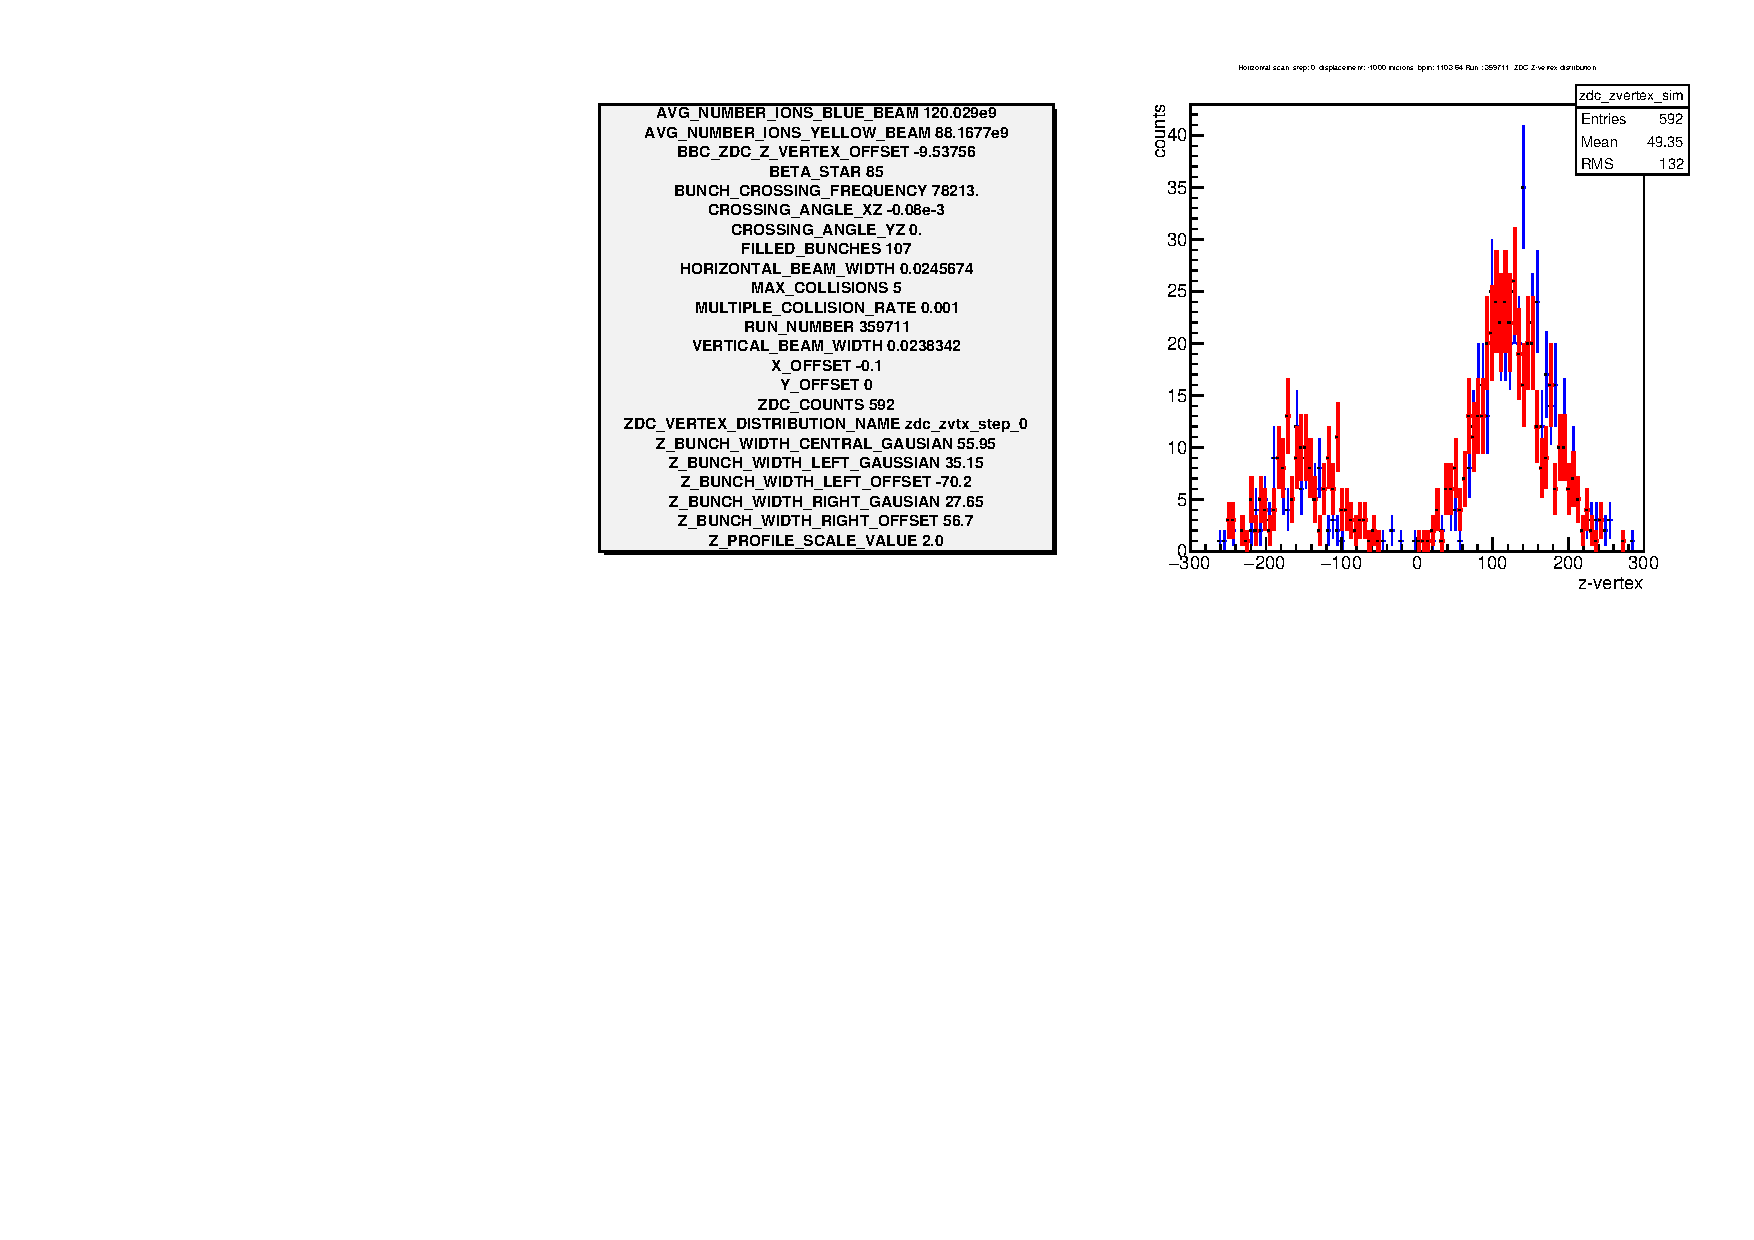
\includegraphics[width=10cm,scale=0.8]{../HourglassResults/figs/359711_step0_config_compare.pdf}
\end{center}
\textbf{Feature:} Good agreement between \textcolor{red}{simulation} and \textcolor{blue}{data}.
\end{frame}

\begin{frame}{359711, -450 micron x-displacement, $\beta^{*} = 85 cm$, $\theta_{xz} = -0.08\times10^{-3}rad$}
\begin{center}
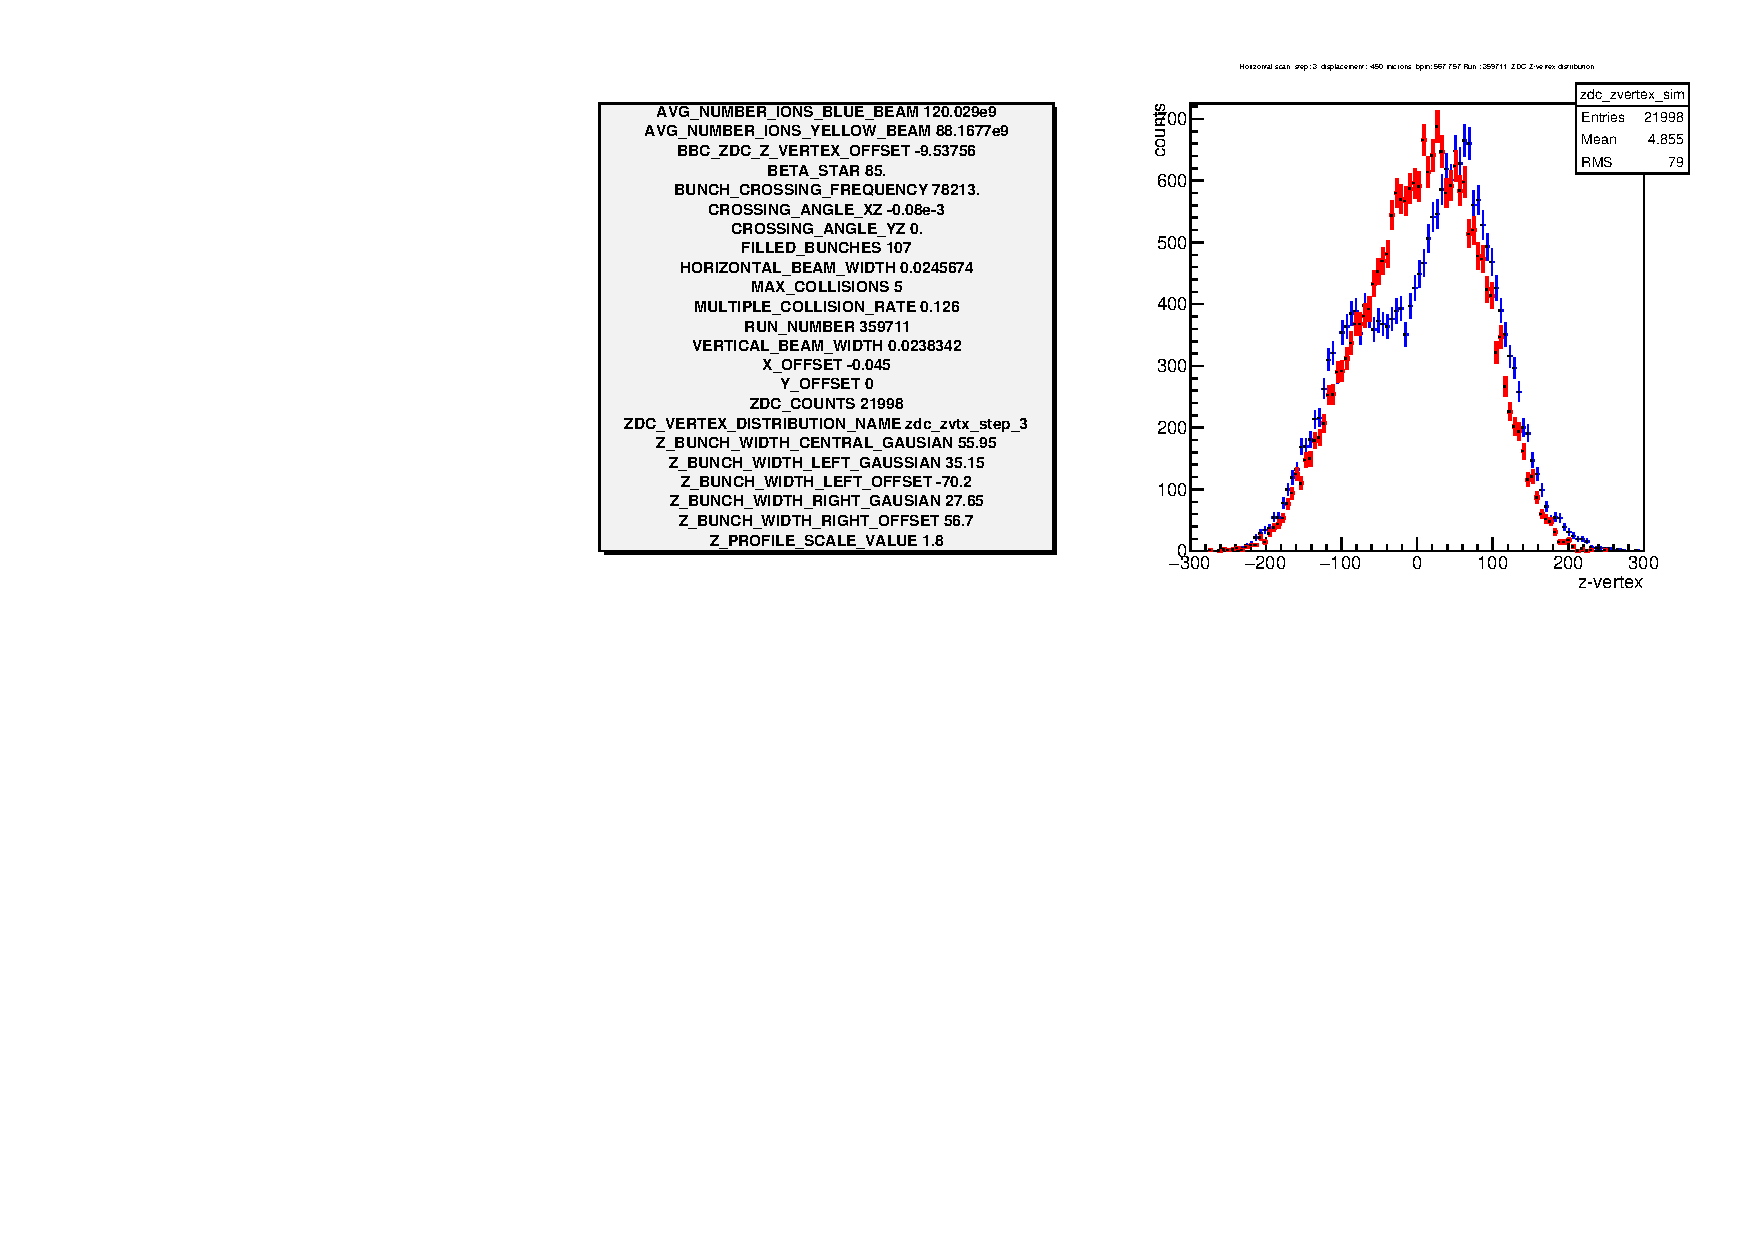
\includegraphics[width=10cm,scale=0.8]{../HourglassResults/figs/359711_step03_config_compare.pdf}
\end{center}
\textbf{Feature:} Closer overlap features are not captured between \textcolor{red}{simulation} and \textcolor{blue}{data}.
\end{frame}

\begin{frame}{359711, -150 micron x-displacement, $\beta^{*} = 85 cm$, $\theta_{xz} = -0.08\times10^{-3}rad$}
\begin{center}
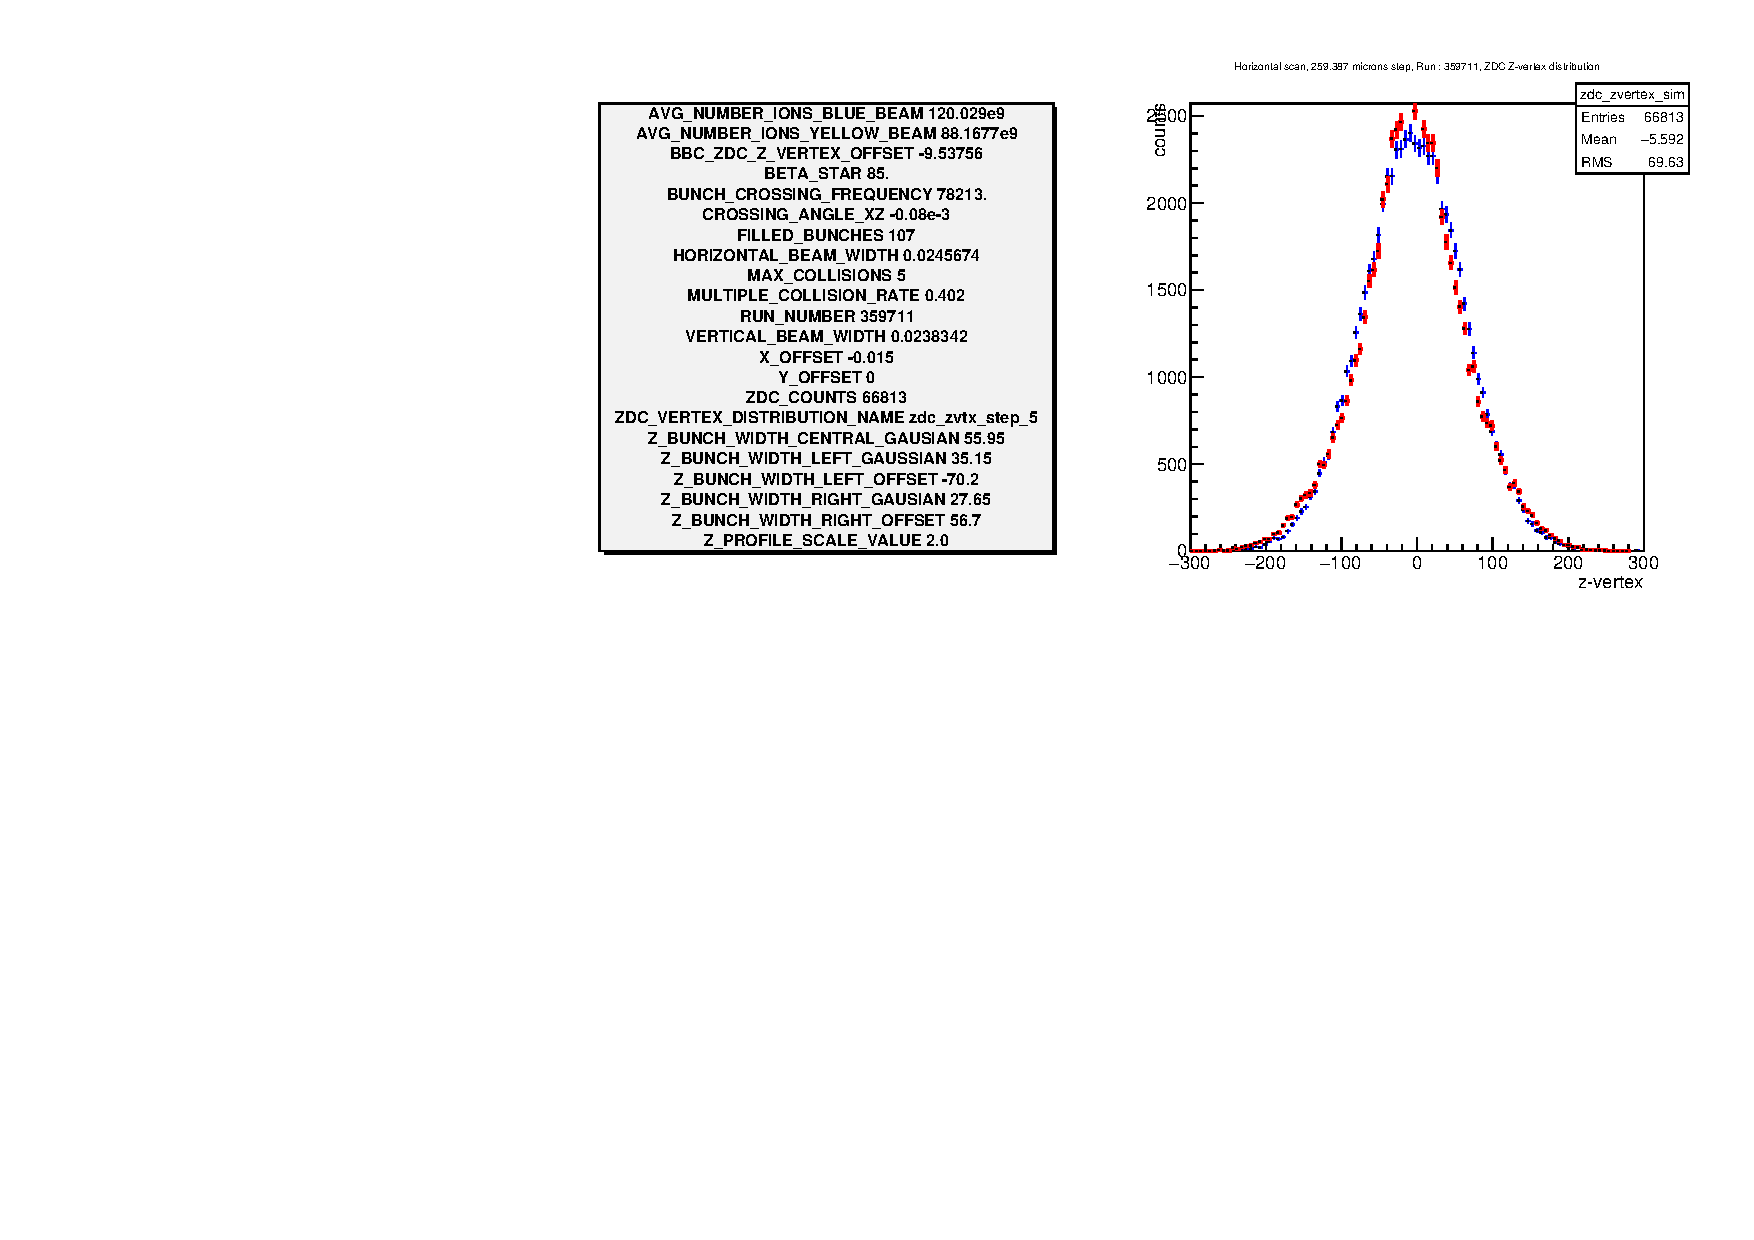
\includegraphics[width=10cm,scale=0.8]{../HourglassResults/figs/359711_step05_config_compare.pdf}
\end{center}
\textbf{Feature:} Good agreement between \textcolor{red}{simulation} and \textcolor{blue}{data}.
\end{frame}

\begin{frame}{359711, -750 micron y-displacement, $\beta^{*} = 85 cm$, $\theta_{xz} = -0.08\times10^{-3}rad$}
\begin{center}
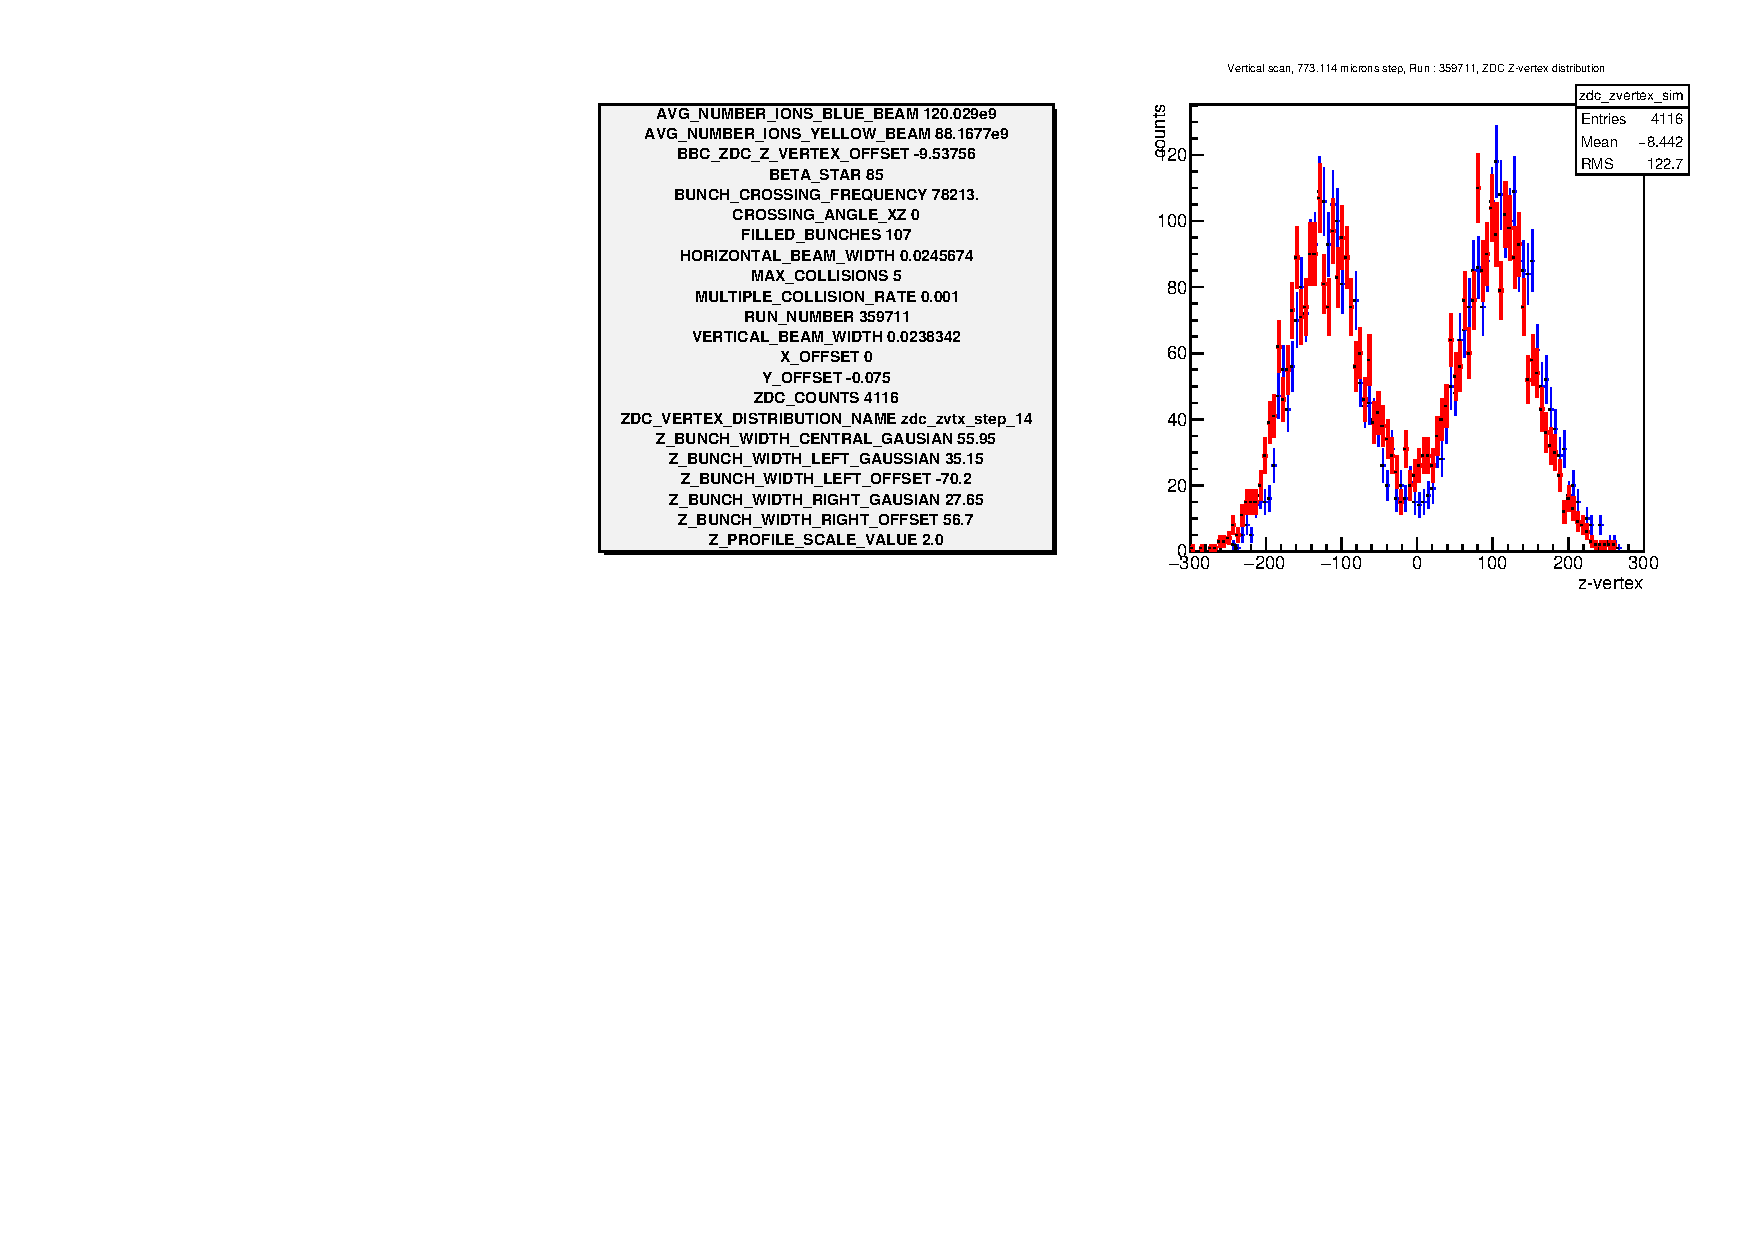
\includegraphics[width=10cm,scale=0.8]{../HourglassResults/figs/359711_step14_config_compare.pdf}
\end{center}
\textbf{Feature:} Apparently, no $\theta_{YZ}$, good agreement between
\textcolor{red}{simulation} and \textcolor{blue}{data}.
\end{frame}

\begin{frame}{359711, 750 micron x-displacement, $\beta^{*} = 85 cm$, $\theta_{xz} = -0.08\times10^{-3}rad$}
\begin{center}
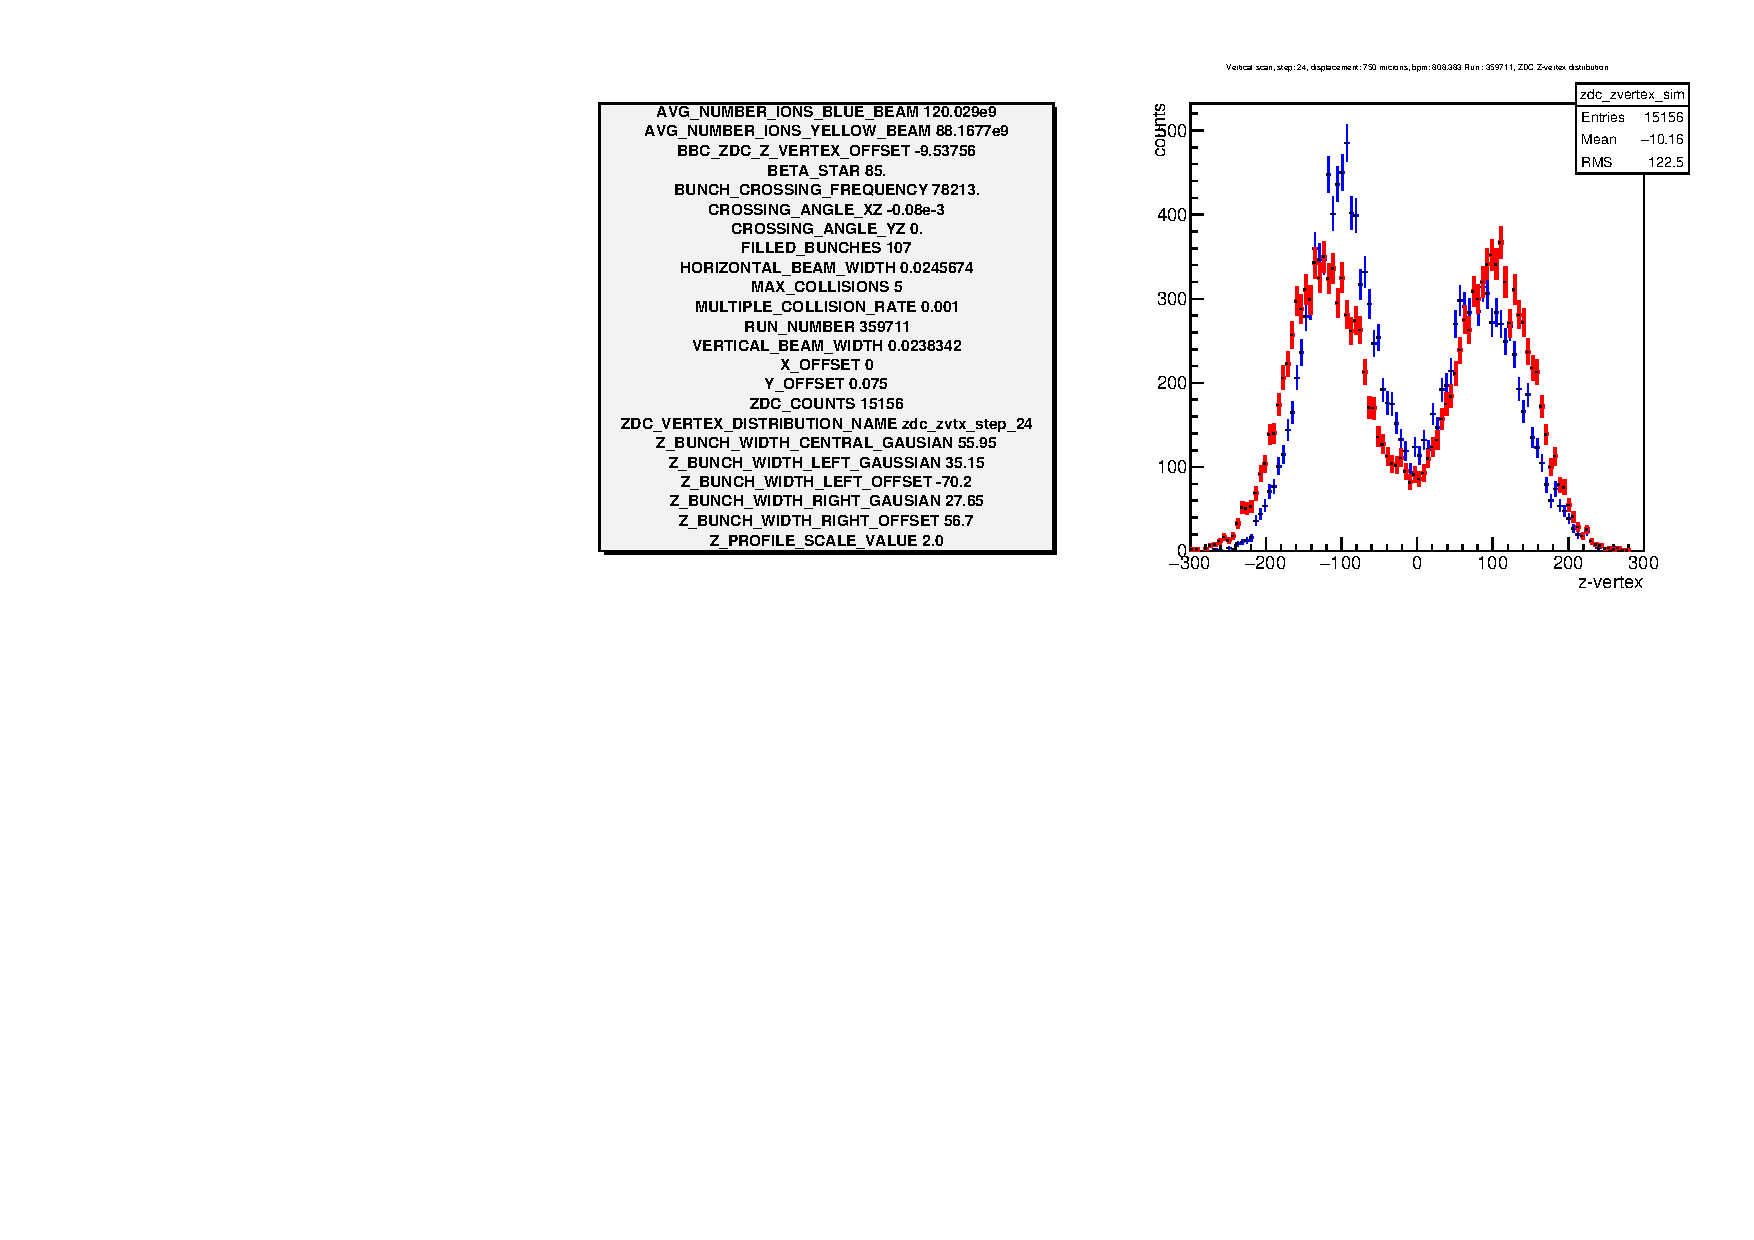
\includegraphics[width=10cm,scale=0.8]{../HourglassResults/figs/359711_step24_config_compare.pdf}
\end{center}
\textbf{Feature:} Data shows presence of $\theta_{YZ}$, makes for poor agreement between \textcolor{red}{simulation} and \textcolor{blue}{data}.
\end{frame}

\begin{frame}{Next Steps Towards More Results}
\begin{itemize}
\item We have already shown that the bunch z-profile affects the z-vertex profile. Is it valid to simply scale this profile?
\item Do we really see a changing crossing angle, or are we seeing fluctuations?
\end{itemize}
These questions can both be answered, but a few things need to happen first.
\begin{itemize}
\item Double check luminosity model (one day)
\item Compare simple models to "real" models (one day)
\item Use "real" bunch z-profile (next slides), compare to current results.
\end{itemize}
\end{frame}

\begin{frame}{Using Z-Bunch Profiles Directly}
This would have been done sooner, but I do not have direct access to the
fine-binned Wall-Current-Monitor data, and there was a 2-3 week lag time in
between requesting the data, and receiving the data.

What I propose:
\begin{itemize}
\item Normalize each profile, to treat it as a density, $\rho_{z}$, such that $\rho(x,y,z,t) = \rho(x,z)\rho(y,z)\rho(z)\rho(t)$
\item Directly use this profile, storing it as a TGraph object and using spline-itripolation to approximate a continuous funciton
\end{itemize}
\textbf{Caveat:} Pictured is the average intensity of each filled bunch, taken
in the middle of a vernier scan.
\end{frame}

\begin{frame}{362492 WCM Z Bunch Profile}
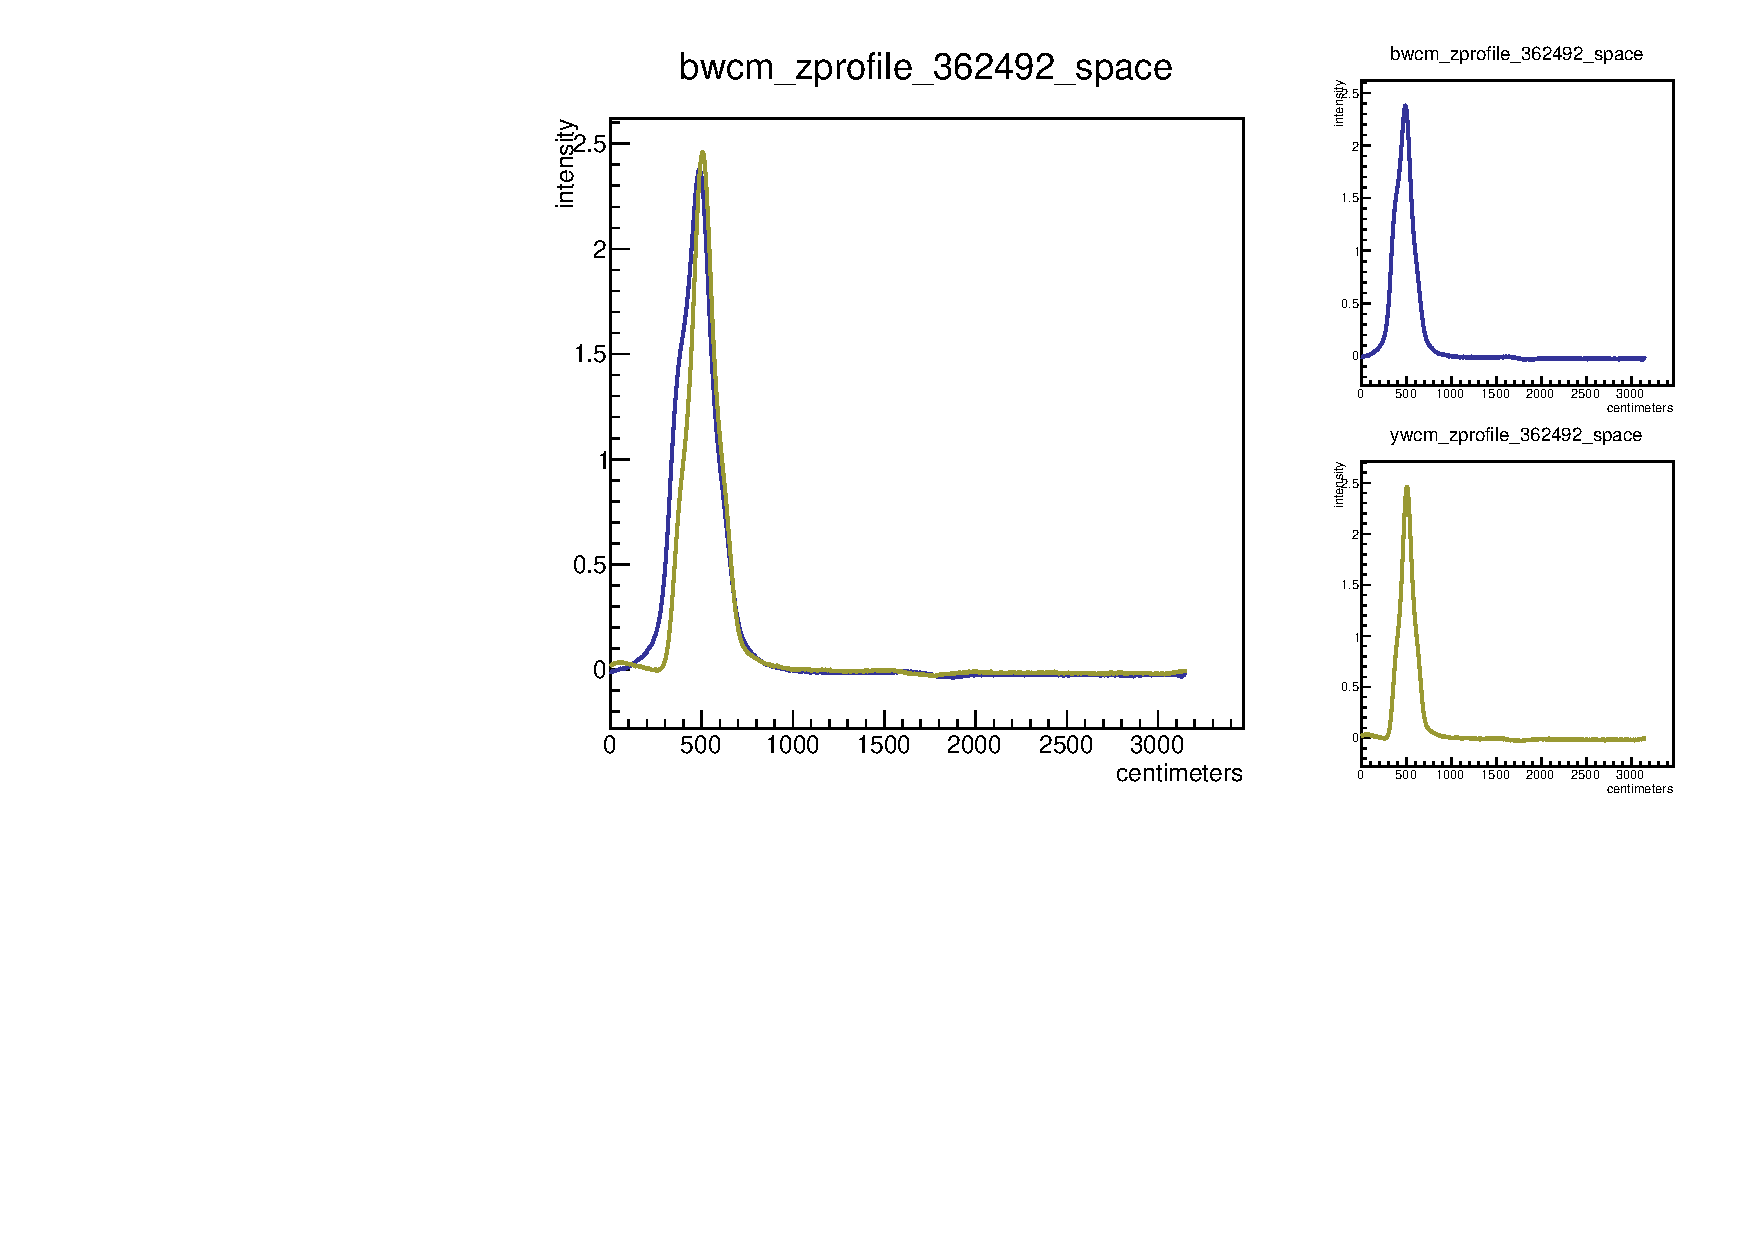
\includegraphics[width=\linewidth,height=\textheight,keepaspectratio]{../HourglassResults/figs/362492_wcm_zprofile.pdf}
\end{frame}

\begin{frame}{365866 WCM Z Bunch Profile}
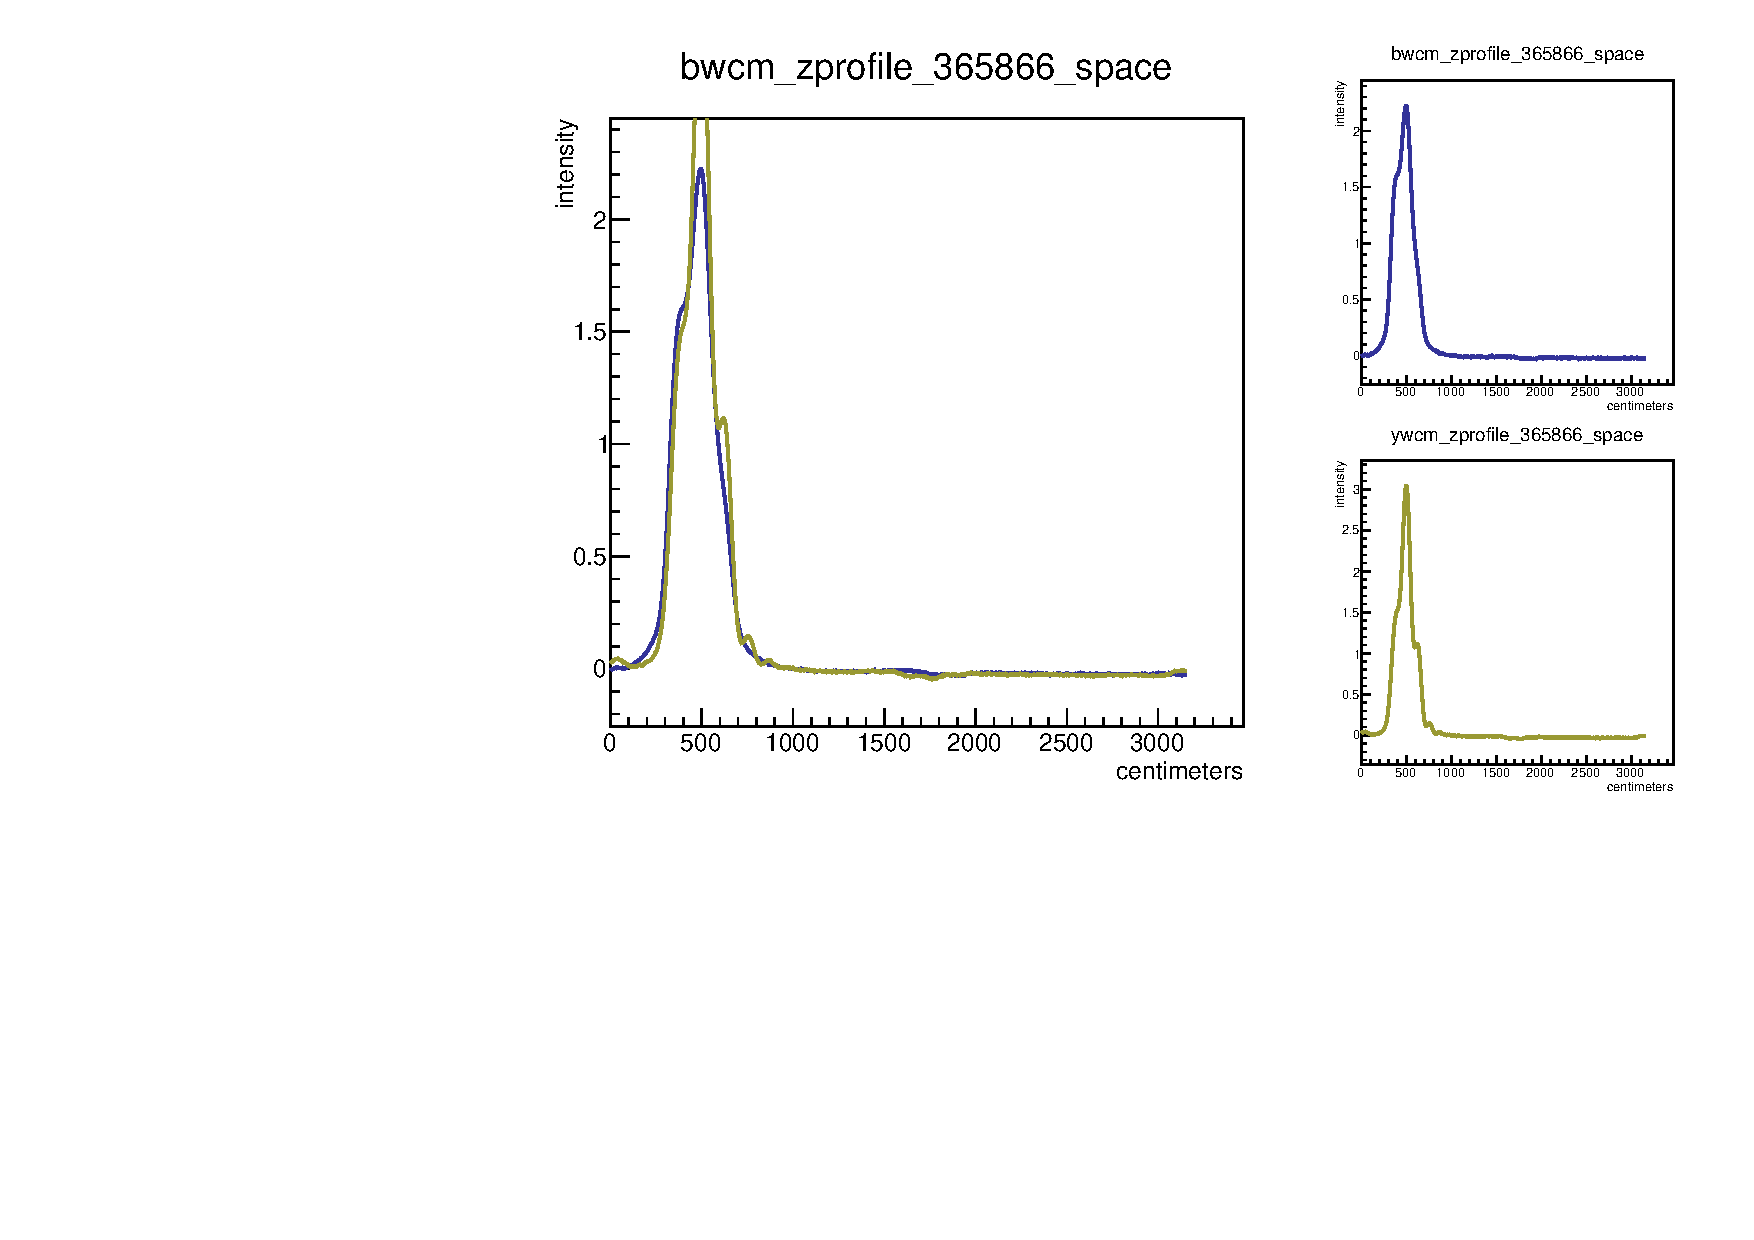
\includegraphics[width=\linewidth,height=\textheight,keepaspectratio]{../HourglassResults/figs/365866_wcm_zprofile.pdf}
\end{frame}

\begin{frame}{366605 WCM Z Bunch Profile}
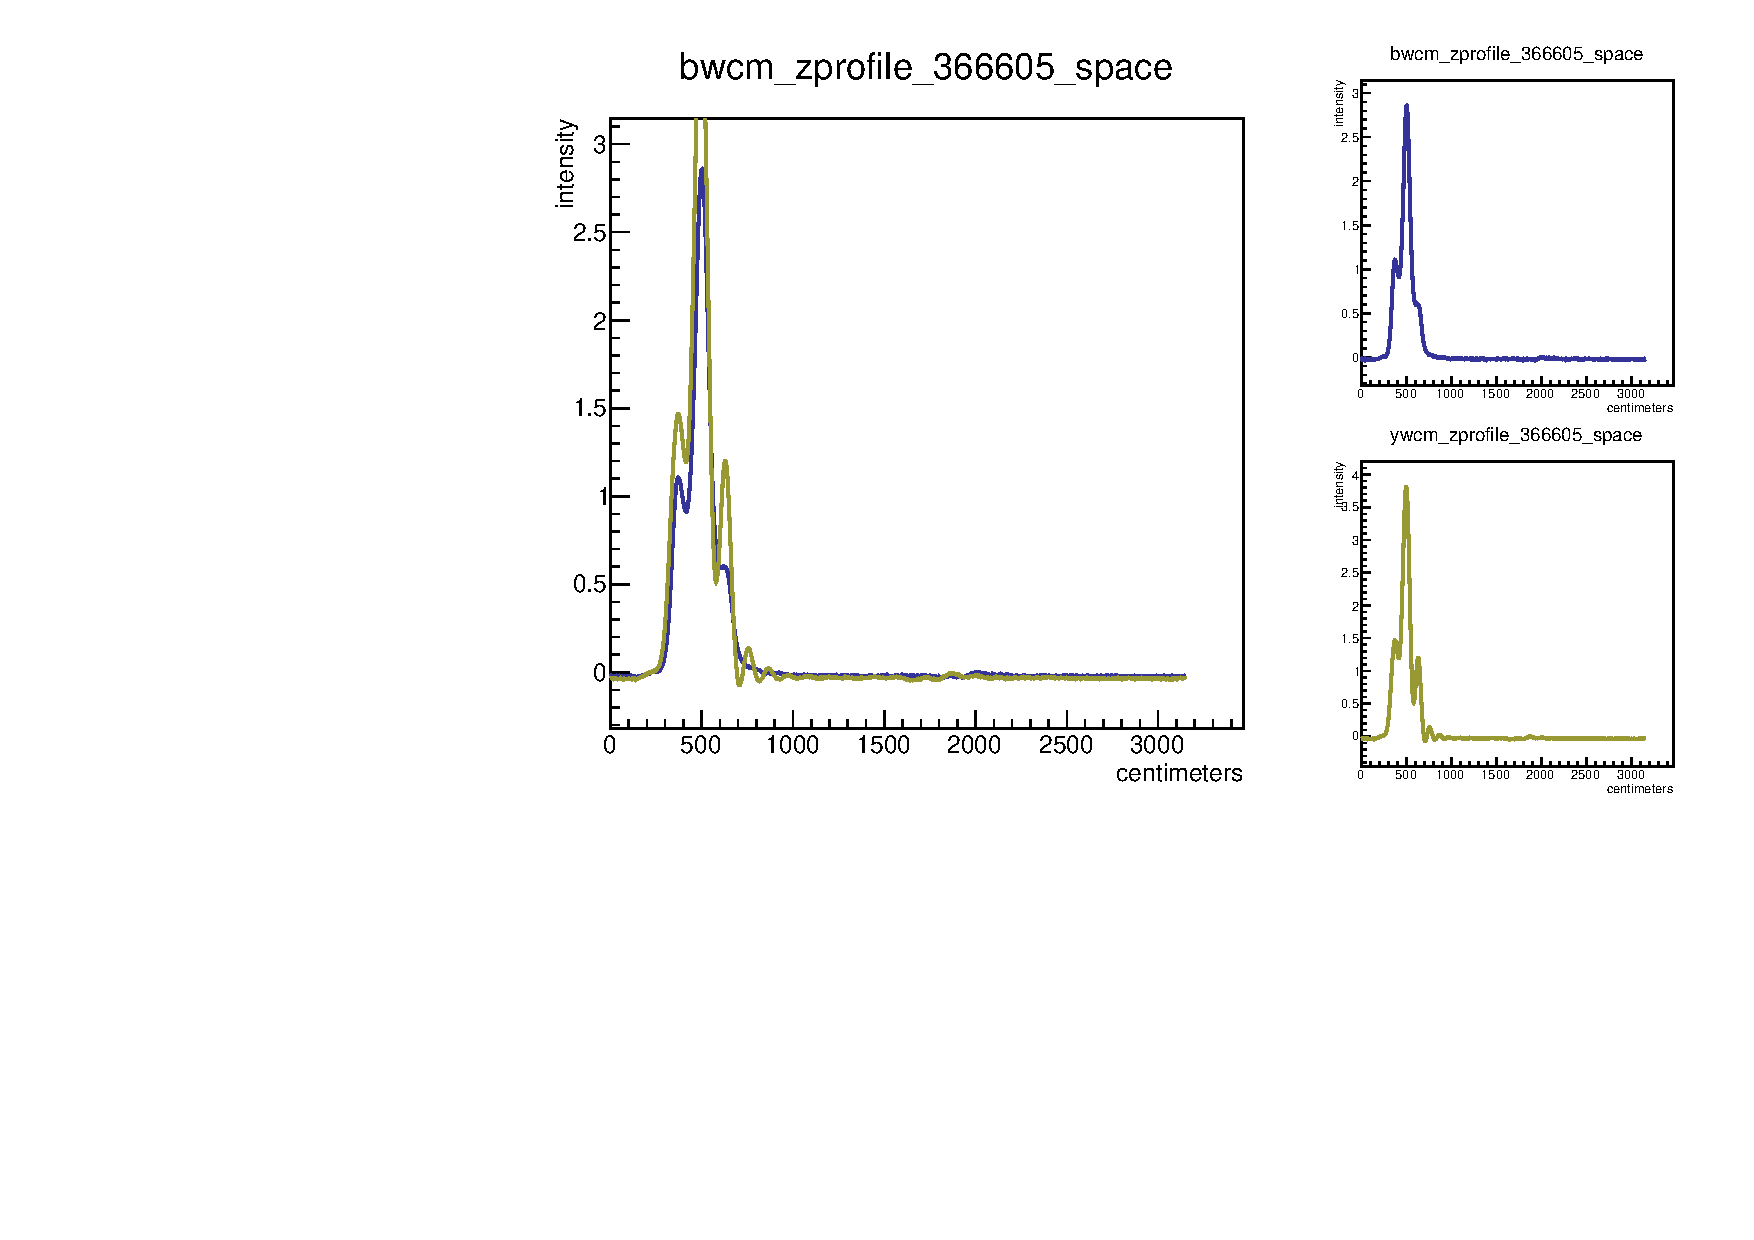
\includegraphics[width=\linewidth,height=\textheight,keepaspectratio]{../HourglassResults/figs/366605_wcm_zprofile.pdf}
\end{frame}

\begin{frame}{364636 WCM Z Bunch Profile}
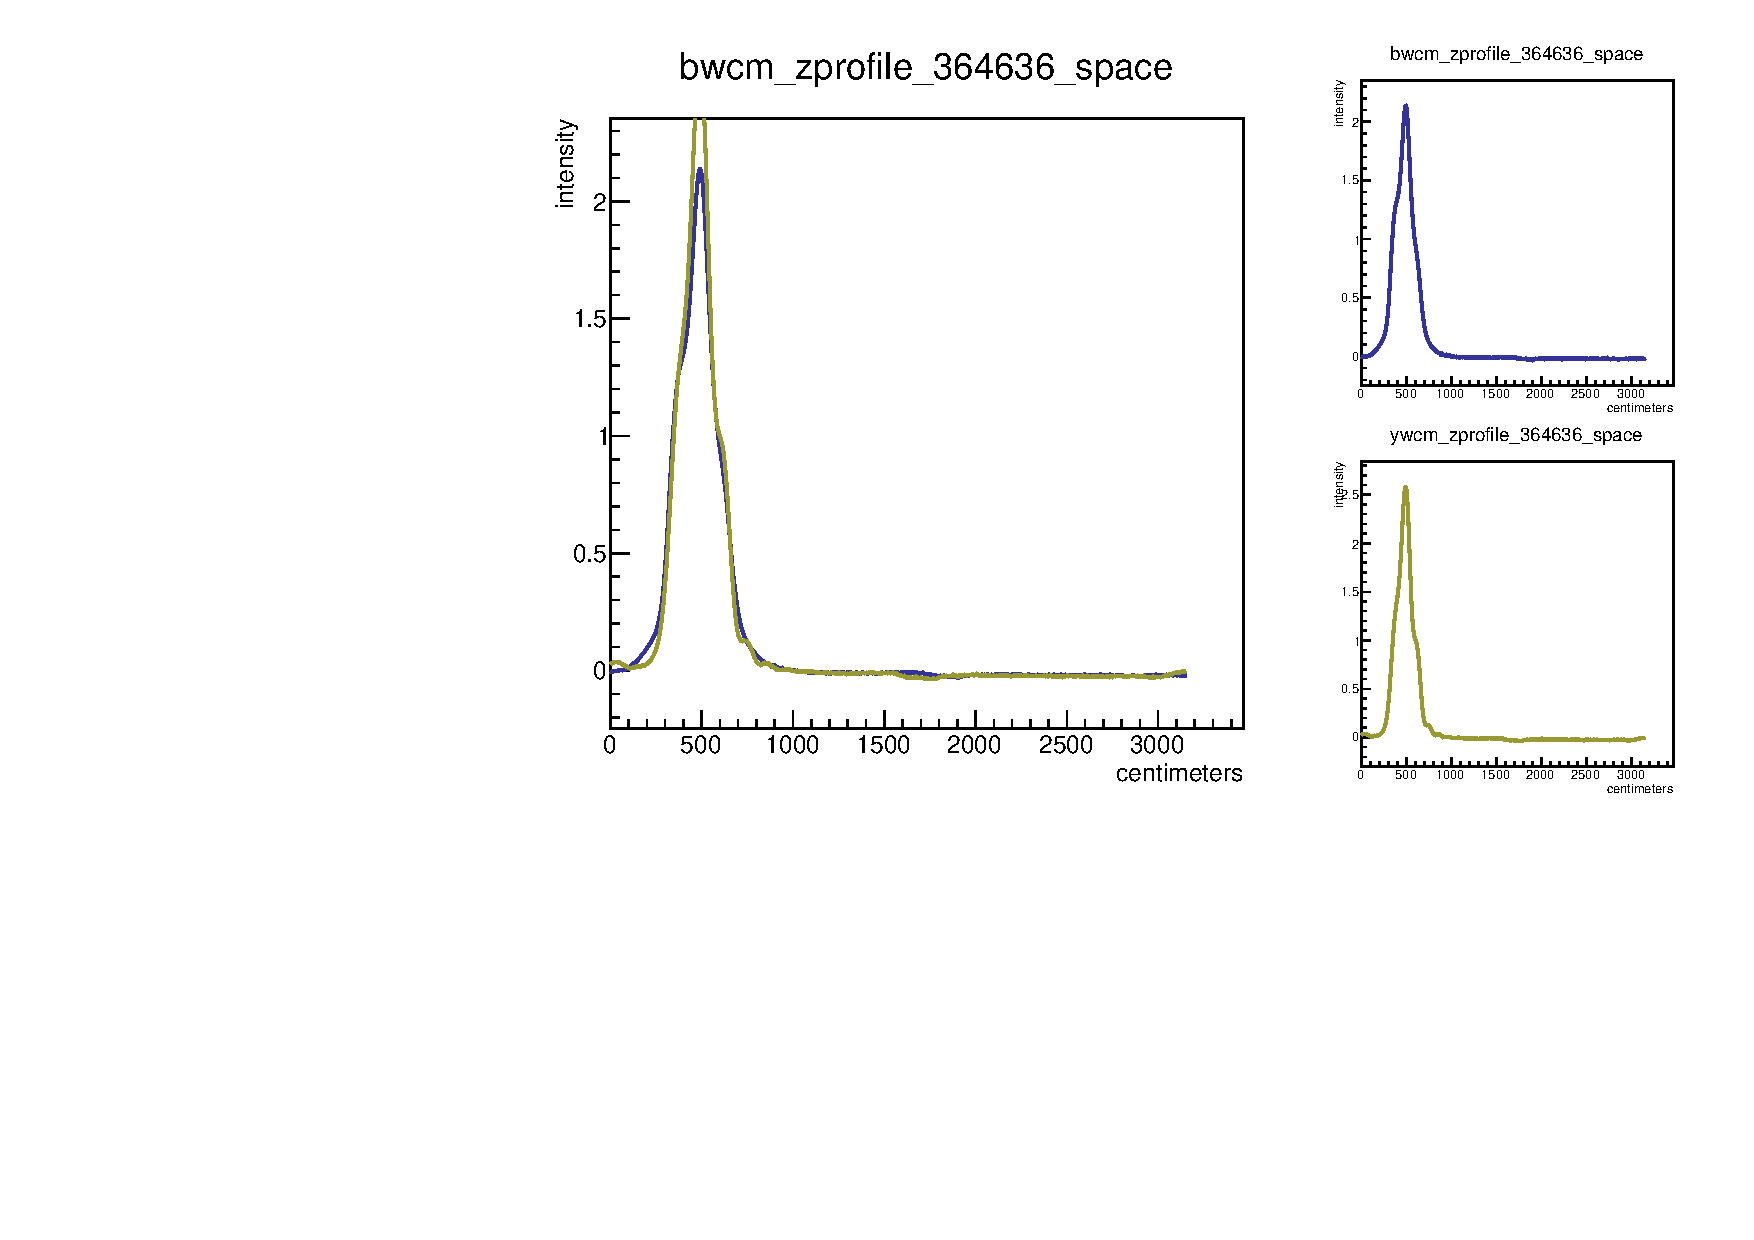
\includegraphics[width=\linewidth,height=\textheight,keepaspectratio]{../HourglassResults/figs/364636_wcm_zprofile.pdf}
\end{frame}

\begin{frame}{359711 WCM Z Bunch Profile}
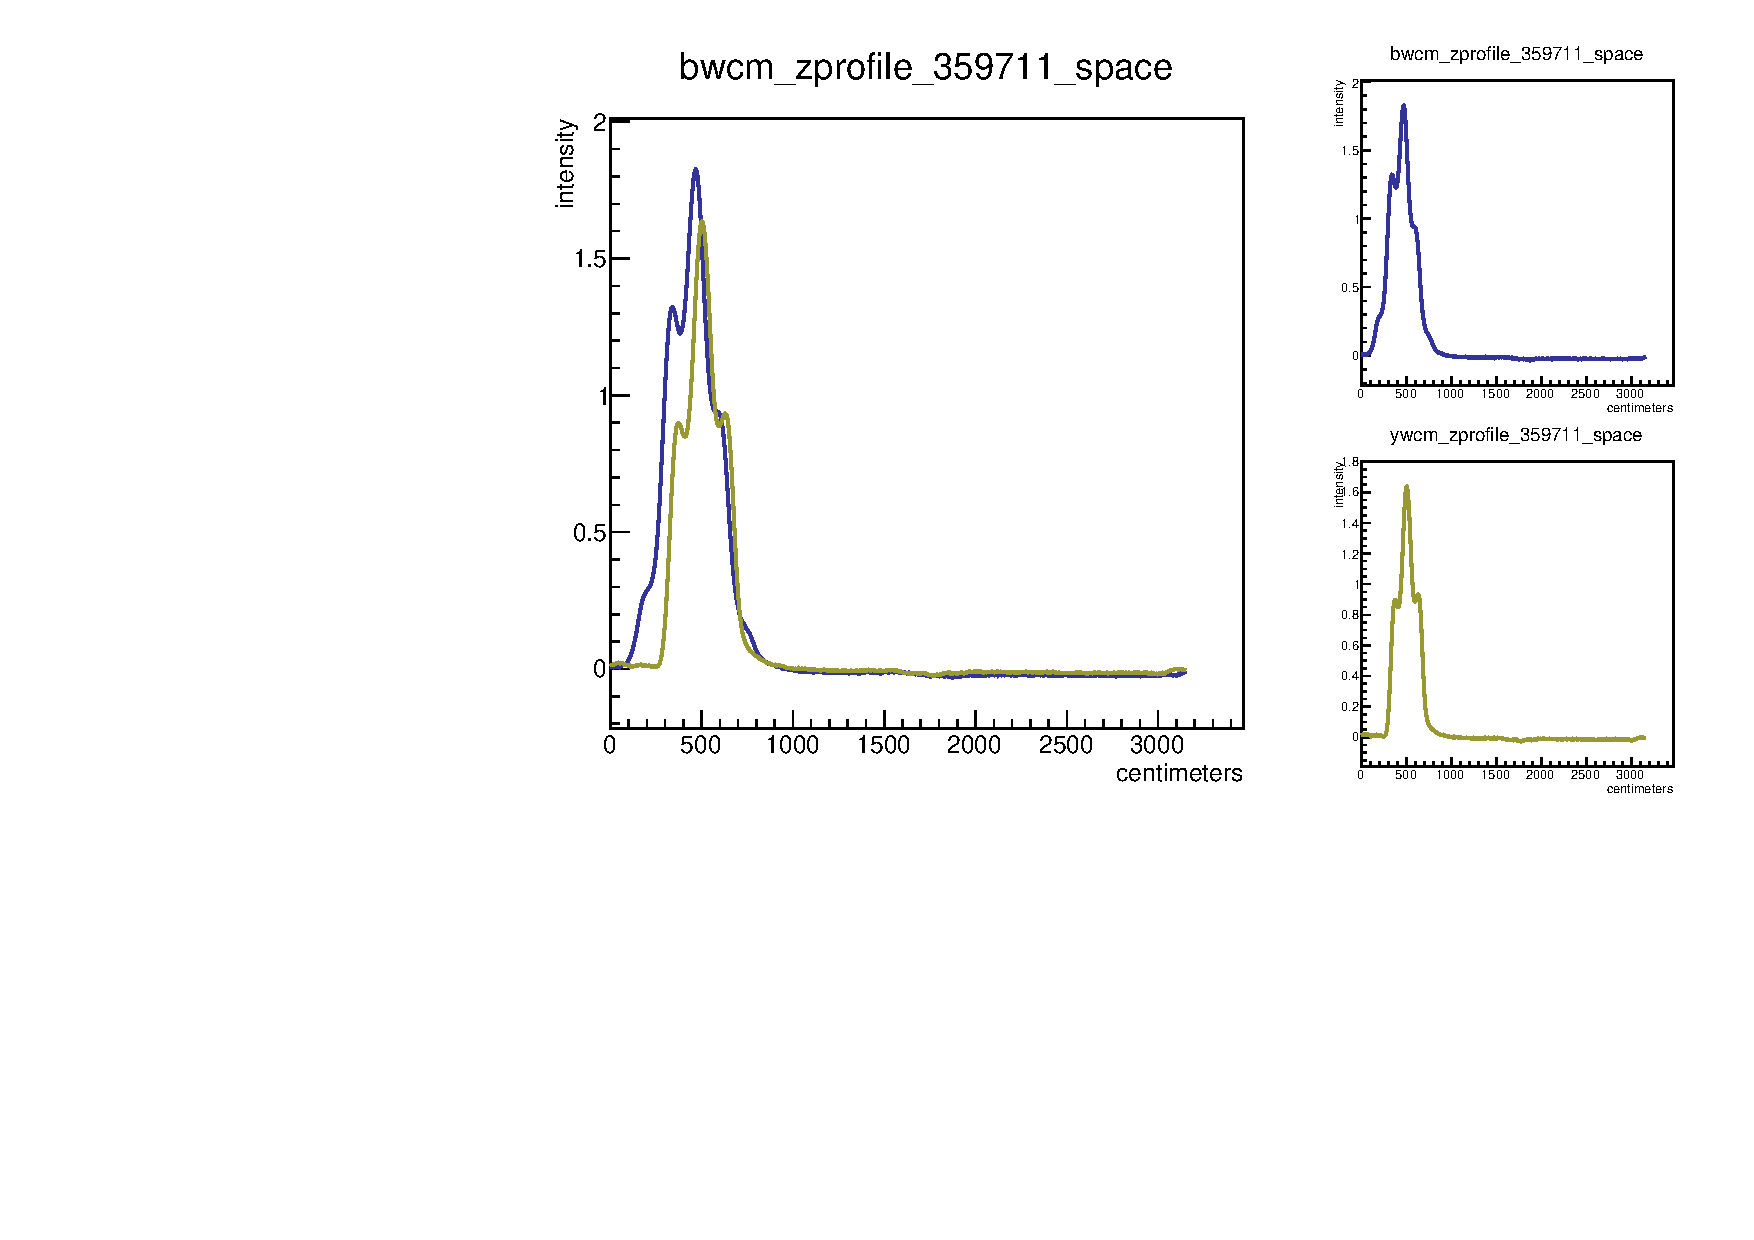
\includegraphics[width=\linewidth,height=\textheight,keepaspectratio]{../HourglassResults/figs/359711_wcm_zprofile.pdf}
\end{frame}

\begin{frame}{367138 WCM Z Bunch Profile}
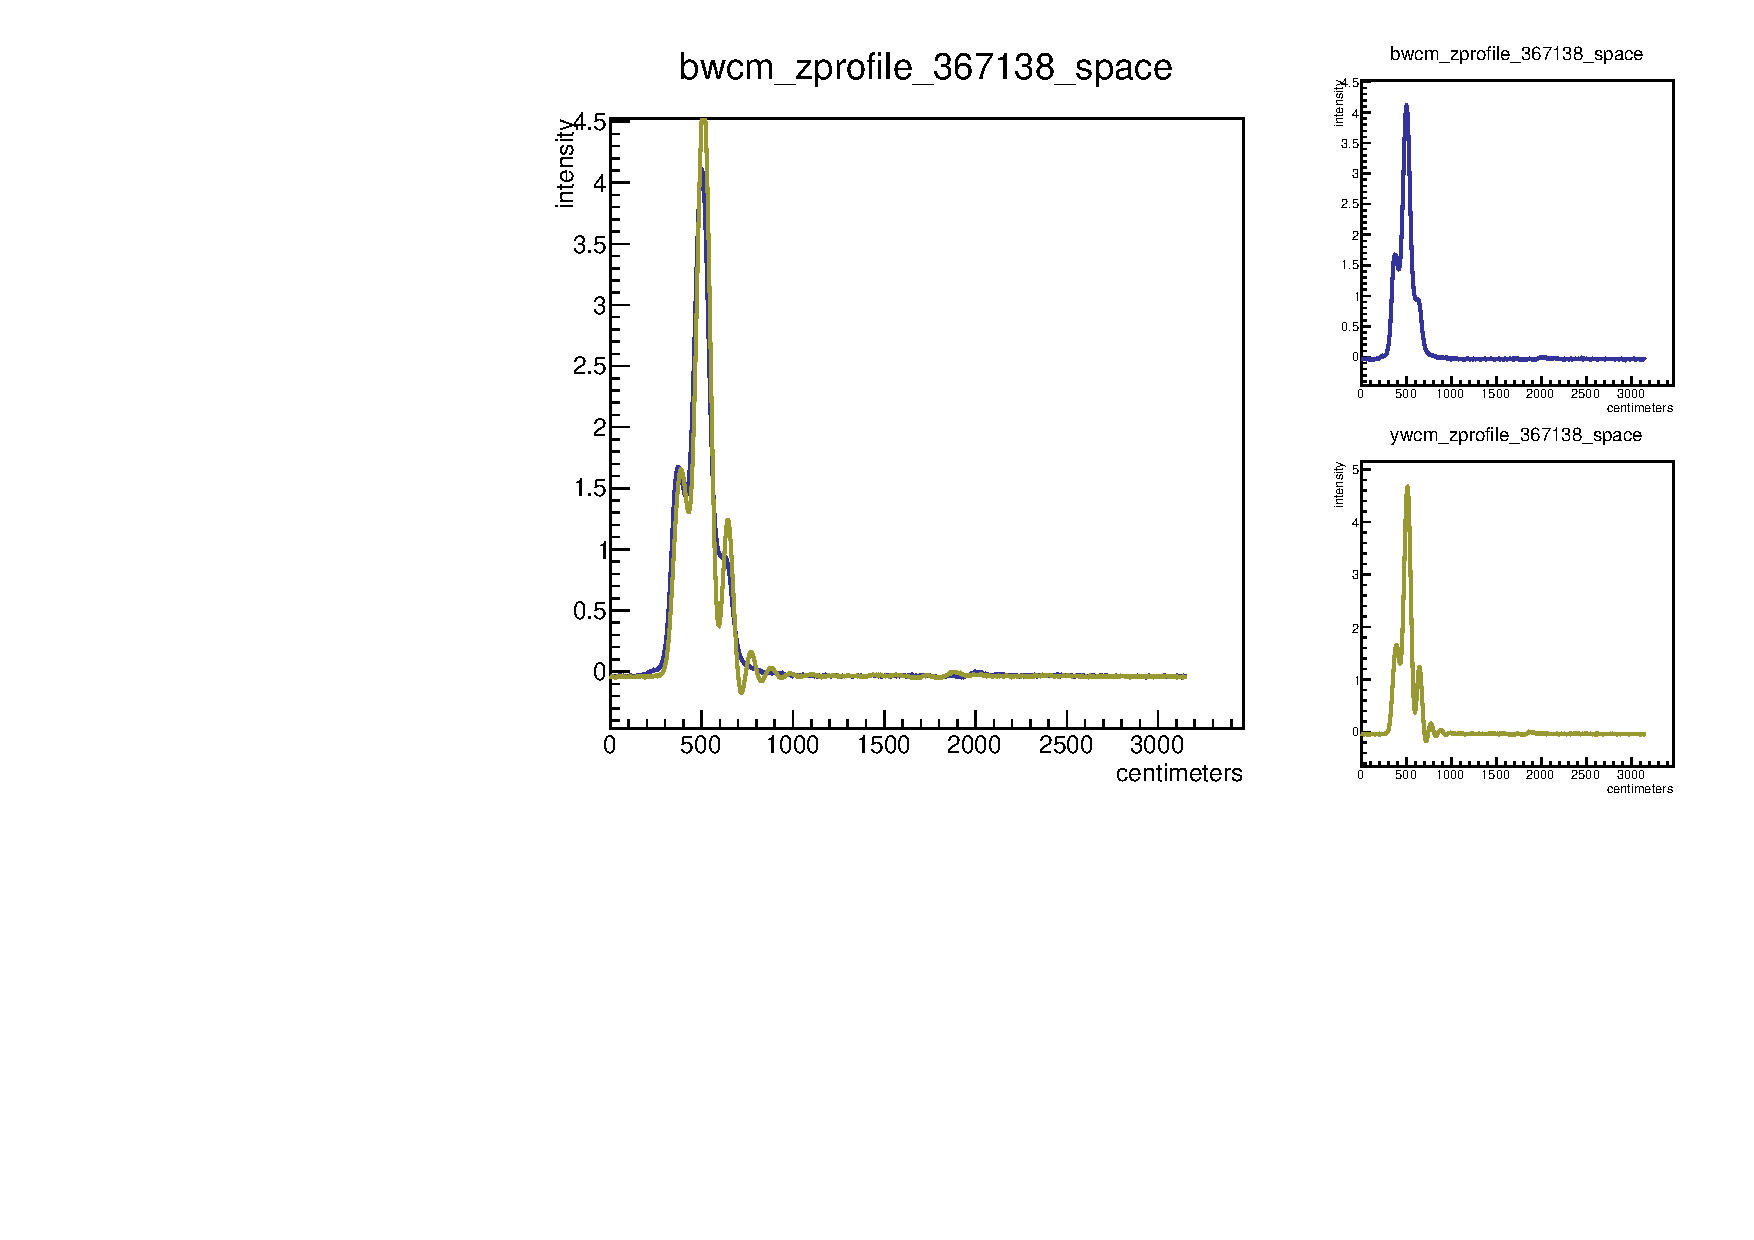
\includegraphics[width=\linewidth,height=\textheight,keepaspectratio]{../HourglassResults/figs/367138_wcm_zprofile.pdf}
\end{frame}

\begin{frame}{360879 WCM Z Bunch Profile}
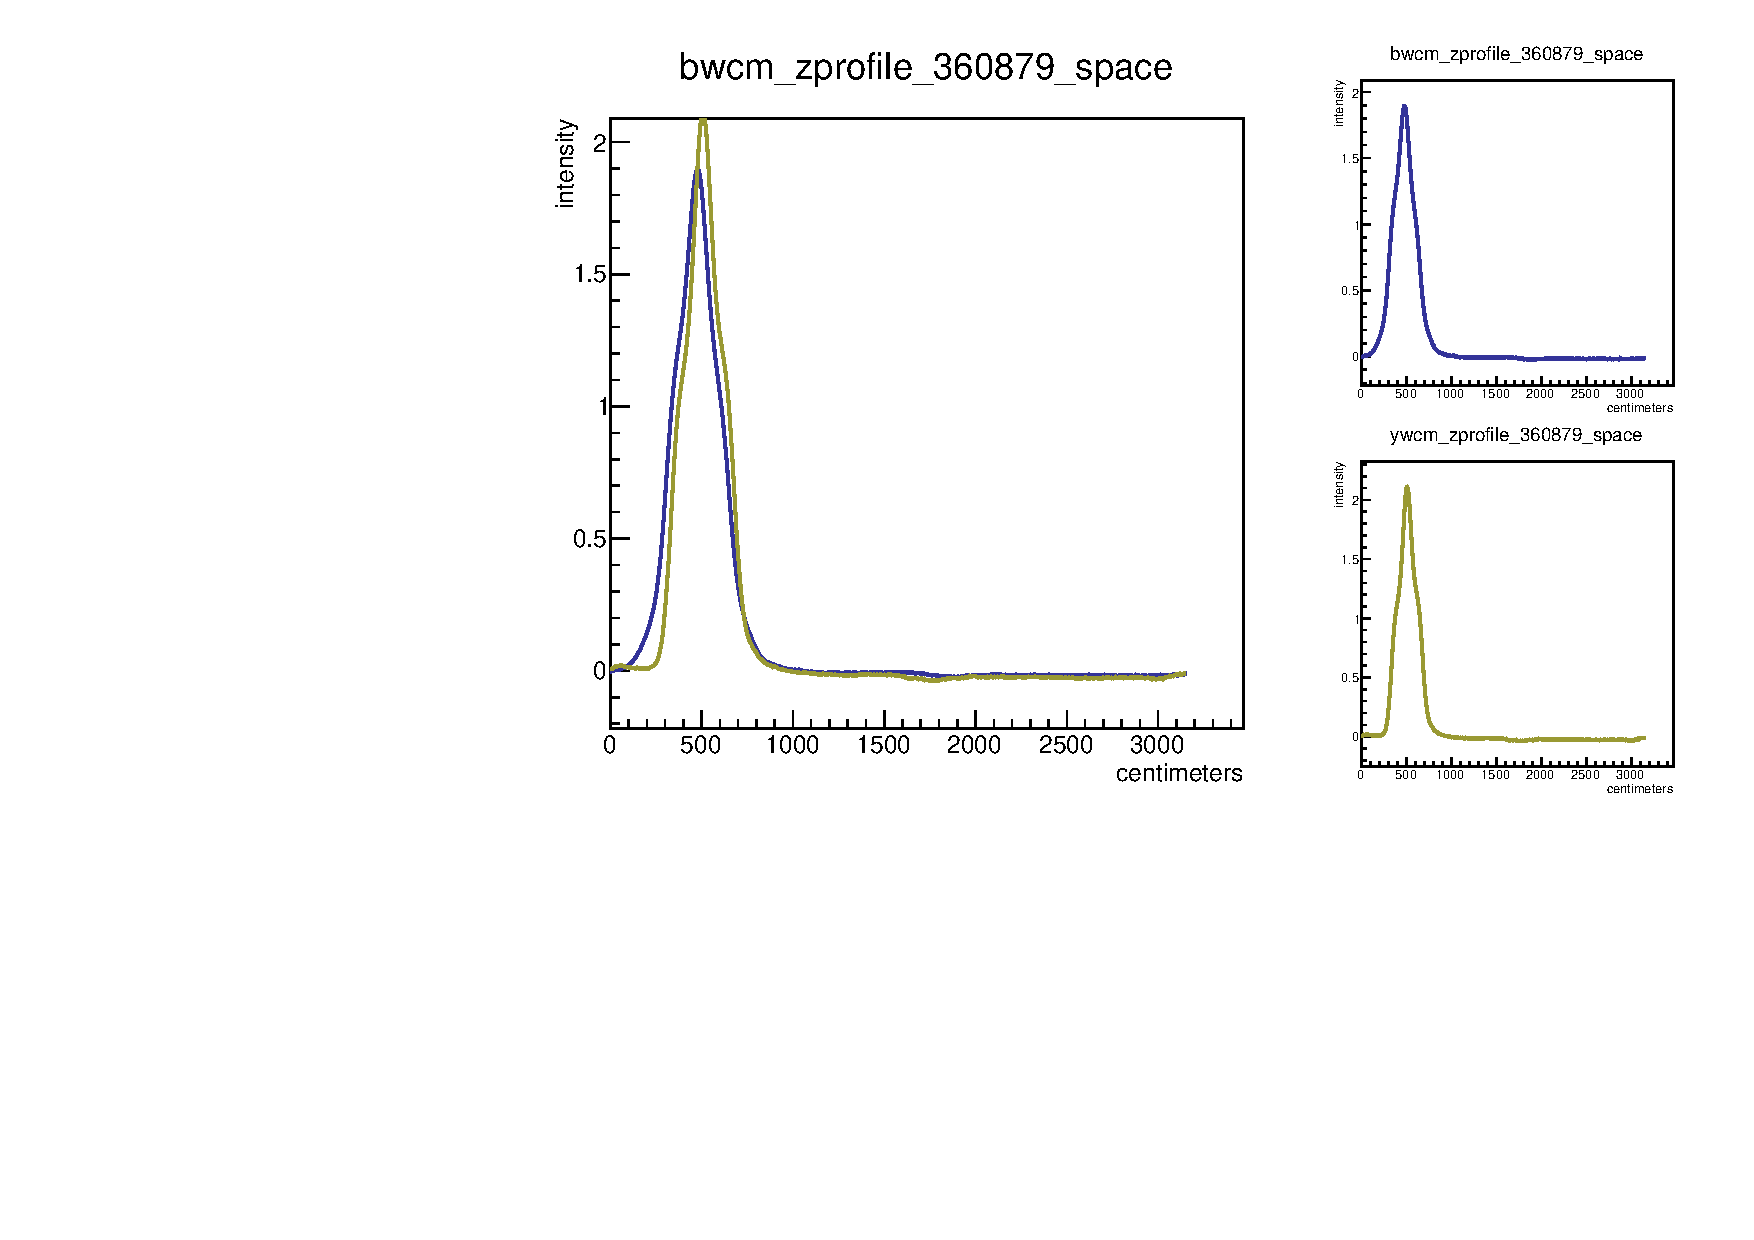
\includegraphics[width=\linewidth,height=\textheight,keepaspectratio]{../HourglassResults/figs/360879_wcm_zprofile.pdf}
\end{frame}

\begin{frame} {Discussion - WCM Z Bunch Profile}
It is clear that sometimes the triple-gaussian profile may be reasonable, but
often it is not. It should not be any problem to substitue in the real profile
into the simulation.
\end{frame}

